\documentclass{article}
% IMPORTANT: path to the figures folder!
%\newcommand{\folder}{C:/Users/../../../figures}

%%%%%%%%%%%%%%%%%%%%%%%%%%
%% Fundamental packages %%
%%%%%%%%%%%%%%%%%%%%%%%%%%

\usepackage{siunitx} 
\sisetup{input-symbols = ()}
\usepackage{array}
\usepackage{amsmath}
\usepackage{amssymb}
\usepackage{amsthm}
\usepackage{extarrows}
\usepackage[normalem]{ulem}
\usepackage[USenglish]{babel}
\usepackage[T1]{fontenc}
\usepackage[utf8]{inputenc}
\usepackage{tgtermes}
\usepackage{ragged2e}
\usepackage{chngcntr}
\usepackage{rotating}


\usepackage{datetime}
\newdateformat{monthyeardate}{%
  \monthname[\THEMONTH] \THEYEAR} % datetime format can be changed, of course

%%%%%%%%%%%%%%
%% Geometry %%
%%%%%%%%%%%%%%

\newcommand{\linesperpagedesired}{35}
\usepackage{pdflscape}
\usepackage[left=3cm, top=2cm, right=2cm, bottom=2cm]{geometry}
\linespread{1.5}
\usepackage{changepage} % needed to make the margins of the Appendix page for additional figures a bit larger
\usepackage{adjustbox}
\usepackage{afterpage}

%%%%%%%%%%%%%%%%%%%%%%%%%%%%%%%%
%% Sections, TOC and appendix %%
%%%%%%%%%%%%%%%%%%%%%%%%%%%%%%%%


%\usepackage{titling}
\usepackage[compact]{titlesec}
\titleformat{\subsubsection}[runin]
  {\normalfont\normalsize\bfseries}{\thesubsubsection}{1em}{}

% if you want to change to spacing of the sections' titles use:
%\titlespacing{\section}
%{0pt}{ex}{4.5ex}

\usepackage[titles]{tocloft}
\renewcommand{\contentsname}{Table of contents}
\renewcommand{\cftsecfont}{\normalfont\bfseries}% titles in bold
\renewcommand{\cftsecpagefont}{\normalfont\bfseries}% page numbers in bold

\usepackage[toc, page, title]{appendix}
\renewcommand\appendixtocname{Appendix}
\renewcommand\appendixpagename{Appendix}
 \renewcommand{\thefootnote}{\fnsymbol{footnote}}

%%%%%%%%%%%%
%% Colors %%
%%%%%%%%%%%%

\usepackage{xcolor}

\definecolor{UBonnBlue}{RGB}{0007,0082,0154}
\definecolor{Occ-A}{HTML}{EB760A}
\definecolor{Occ-B}{HTML}{43AA8D}
\definecolor{Edu}{HTML}{F9C74F}
\definecolor{Home}{HTML}{577590}

%%%%%%%%%%%%%%%%%%%%%%%%
%% Figures and tables %%
%%%%%%%%%%%%%%%%%%%%%%%%

\usepackage{booktabs}
\usepackage{longtable}
\usepackage{multirow}
\usepackage{graphicx}
\usepackage{subcaption}
\usepackage[labelfont=bf]{caption}
\usepackage{tabularx}
\usepackage{float}
\usepackage[edges]{forest}
\usepackage{tikz}
\usetikzlibrary{shapes,positioning,arrows.meta,calc,patterns}



\numberwithin{figure}{section}
\numberwithin{table}{section}
\setlength{\parindent}{0in}

%%%%%%%%%%%%%%%%%%%%%%%%%%%%%
%% Theorems and definition %%
%%%%%%%%%%%%%%%%%%%%%%%%%%%%%

\makeatletter
\newtheoremstyle{indented}
  {3pt}% space before
  {3pt}% space after
  {\addtolength{\@totalleftmargin}{3.5em}
   \addtolength{\linewidth}{-3.5em}
   \parshape 1 1.5em \linewidth \itshape}% body font
  {}% indent
  {\bfseries}% header font
  {.}% punctuation
  {.5em}% after theorem header
  {}% header specification (empty for default)
\makeatother


 {
      \theoremstyle{indented}
      \newtheorem{assumption}{Assumption}
      \newtheorem{definition}{Definition}
      \newtheorem{proposition}{Proposition}
  }


\numberwithin{equation}{section} % number equations within
								 % section and subsection

\newcommand\stab[1][0.45cm]{\hspace*{4.5 mm}} % tab needed for formulas in   												  % proof in appendix

%%%%%%%%%
%% URL %%
%%%%%%%%%

\usepackage{hyperref}
\hypersetup{
	colorlinks = true,
	linkcolor = black,
	urlcolor = black,
	citecolor = UBonnBlue,
	}

%%%%%%%%%%%%%%%%%%%
%% Bibiliography %%
%%%%%%%%%%%%%%%%%%%

\usepackage{natbib}
\bibliographystyle{unsrtnat}
\renewcommand{\bibsection}{\section*{References}}
%\DeclareLanguageMapping{english}{english-apa}
%\setcounter{biburlnumpenalty}{85}
%\addbibresource{bibliography.bib} % .bib file has to be in the same directory of this file
\renewcommand{\UrlFont}{\small\ttfamily}



\title{\textbf{Research Proposal} \\ Word-of-Mouth Communication in Digital Markets}
\author{Iana Gerina \footnote{University of Vienna (VGSE),  \href{mailto:iana.gerina@univie.ac.at}{iana.gerina@univie.ac.at}}}
\date{\today}

\begin{document}

\maketitle
\thispagestyle{empty}
%2-4 pages without bibliography

\begin{center}
    \textbf{Abstract}
\end{center}


\vspace{6ex}
\textbf{Keywords}: Vertical differentiation, word-of-mouth communication, digital markets. 


\clearpage
\section{Introduction} \label{motivation}

In this research proposal I outline three projects, which are aimed at investigating the multi-faceted effects of the word-of-mouth communication on the digital markets outcomes, including product differentiation, market power and entry. This over-arching theme of the dissertation belongs to a wider branch of research on digital markets and WOM communication, and the motivation to study this particular topic is in its novelty and increasing applicability. Each year the amount of shopping online grows by 3-4\% in European countries, and the pandemic is pushing this number even higher.According to 2021 Europen E-Commerce Report, E-GDP of Europe has now reached 3.98\% of the total European GDP.  

With many markets being driven by word-of-mouth and reputation, all digital markets will retain an additional aspect of information exchange due to them being a part of the world-wide web. The influence of word-of-mouth commmunication on market outcomes, as well as the ability of the producer to optimally intervene in it has been studied extensively \citep{Mayzlin2006, Godes2009}, however, much less attention has been given to marketplaces, which by themselves allow consumers to communicate directly with each other \citep{Godes2004} and, especially, the sellers. In my first two projects I focus mainly on software development markets, which are realised through special software development forums, where anybody can post their custom software and receive feedback, thus allowing communication of consumers not only between themselves or with sellers, but even directly with the producers of software. 

The main advantage of and motivation for looking at this type of markets in particular is the fact that they combine specific features of digital apps markets, such as zero pricing and paying for access to good, instead of its quantity, with the aforementioned WOM communication aspects, complete with the possibility of being able to track those perfectly. Focusing on this type of markets then allows me to add new insights to the digital app markets literature by shedding light on the normally unobserved communication between consumers, as well as normally missing communication between them and the producer, adding a new dimension to the existing literature.

The mechanisms behind digital apps markets functioning continue to be a highly topical issue. Digital markets, in general, presented researchers with a number of new market formations, such as digital platforms \citep{Just2018, Choi2021, Appel2020}. Explaining the often surprising market outcomes, e.g. prevalence of zero-price markets, coexistence of free and paid versions ("freemium"), transparency of product development despite it being a public good has long been a prevalent branch of literature \citep{Appel2020, Ajorlou2018}, as well as a vital tool for making informed policy decisions. The aim of my future dissertation is to provide additional insights into the workings of and conditions in these markets at the startup level, as well as the role of consumer-consumer and consumer-producer information exchange within them.

In the second section of the research proposal I describe the first project, which focuses on the dual impact of WOM communication on the quality development decision of a start-up with an innovative idea. From the side of the demand delayed diffusion of information about the new good ensures that some consumers are being kept captive by the incumbent firm, influencing market compeition \citep{Fainmesser2020}, whereas from the side of supply newly attracted consumers provide additional feedback on the product's quality, making the costs of producing better quality product lower. On the other hand, due to the product's development transparency, all entering firms can emulate the incumbent's good entering level of quality without any additional costs. This trade-off, I argue, results in a dual effect from the WOM communication on the market outcomes. While the pricing of the incumbent is that of the monopolist due to the demand-side effects, supply-side effects promote the good's quality development.

The ability of the producers to learn from their feedback is akin to the learning-by-doing effects \citet{Tirole}, as promoting higher demand in the first period results in more demand and thus, more feedback. In this way the project investigates the highly curious outcome of the digital app markets: quality development, despite the transparency and possibility of plagiarism; as well as highlighting an additional incentive to engage in zero pricing even in highly monopolised markets, adding to the standard explanation of zero marginal costs of production \citep{Ajorlou2018, Campbell2015}. In contrast to most classic learning-by-doing and knowledge spillovers literature \citep{Tirole,  Jovanovic1994}, I show that investment in quality is not hindered by learning-by-doing externality due to higher customer base effect (similar to \citet{Jovanovic1994}) and feedback effect.

The simple two-stage model together with simplistic assumptions on the consumer network provides an intuitive way to demostrate the long-term effect of WOM communication. Instead of focusing on the producers optimising their prices in a dynamic setting like \citet{Ajorlou2018}, who provide a framework to explain fluctuation of prices and the frequent zero-pricing, I focus on the market where the zero-pricing is much too pervasive to be a short-run decision, but rather a reaction to a state of the incumbent. Until the state changes, i.e. the incumbent is able to penetrate the market, her price does not fluctuate, but stays zero. In this way the model allows to simply, but efficiently aggregate the effects in the market by using a small number of parameters of interest.

There are two main research question that I address in this project: how does the communication between consumers and producers in a digital marketplace influence the investment of firms in quality of their goods? What is the mechanism behind WOM communication's impact on market monopolisation? To better understand these effects, as well as to quantify their impact, I develop a structural model of price competition in a vertically differentiated market and use the web-scraped data from a software development forum to estimate its parameters. My intention is to disentangle the two effects from each other and provide a number of counterfactuals that illustrate the advantages and disadvantages of the current market equilibria in a number of "but-for" scenarios. 

WOM communication as a driver for product quality has been examined in \citet{Godes2017}. The paper in question predicts a different optimal product-policy response to the growth in social interactions between consumers, depending on whether the structure of the network changes or if it only expands. Building on these results, I aim to investigate the impact of the combination of the feedback effect and the structure of WOM communication. Would a WOM communication network different from the one we observe in the data result in different product-policy decisions? 

In the third section of the proposal I turn to the perspective of the entrant. Whereas it is true that in the short-run no entering firm can compete with the incumbent, in the long-run accumulating a big enough number of consumers an entrant can become the incumbent's competitor, instead of a price-taker. Setting up the second project I argue that this outcome occurs due to increasing returns to scale resulting from the feedback of consumers, as well as special forms of WOM communication networks, which result in market segmentation. 

The idea that WOM communication is a driver behind new product's adoption was proven to be true by \citet{Hill2006}, who showed that being connected to somebody who has adopted the service makes a consumer 3-5 times more likely to adopt it herself. However, as I demonstrate in the first project, delayed information diffusion through WOM communication can lead to market monopolisation. The research question that I want to address with this project is: what is the underlying mechanism of succesful entry in digital markets with WOM communication? To investigate it I formulate a structural model that I will use to estimate the threshold number of consumers that a firm must attract for its entry to be successful in the long-run. Moreover, I examine how this threshold varies depending on the WOM network structure and provide counterfactuals to demonstrate that some types of WOM networks result in natural barriers to entry. 

Finally, in the fourth section of the proposal I describe the third planned project, in which I propose to look into the means that the entrant can employ to overcome the delayed diffusion of information in the long-run, namely promoting WOM via setting a lower price or engaging in advertising auctions. I set up a simple model that explains the trade-off between those two options and illustrate using data how this decision is made. 

%\textbf{Hypothesis:} The market consists of a small number of dominant firms, who have market power, as well as a large number of fringe firms, who are price-takers. This market outcome is due to WOM being doubly advantageous to the dominant firms and restricting the growth of fringe firms, thus resulting in natural barriers to entry. However, due to software development process being transparent to everybody, it also results in higher levels of investment in quality, as long as the market is not completely disjointed.

%However, in contrast to earlier literature I argue that in such markets, where WOM is present, marginal costs of production are not only non-zero, but also negative and decreasing in the number of consumers. In combination with WOM effects on demand, I explain how these characteristics result in the  outcomes I observe in such markets. Moreover, I investigate the properties of the WOM network in software development forums and describe their role in the process of market monopolisation, as well as quality development.


%My aim is to empirically disentangle the two effects on the market outcomes: the WOM communication leading to captive consumers and the effect of feedback on quality development resulting in reduction of costs of production for the entrant. By estimating a structural model I hope to investigate the following counterfactuals: 

%\begin{enumerate}
 %   \item "but for" feedback effect, would the incumbent still be interested in increasing the quality production? 
  %  \item would different structures of WOM communication network result in different market outcomes, e.g. less monopolisation of the market or lower quality investment?
%\end{enumerate}

\setcounter{tocdepth}{2}
\addtocounter{page}{-1}


\section{WOM and vertical differentiation in software development markets}


\subsection{Fundamentals of the Model} \label{model}
 
 In this section I set up a simple two-period game between incumbent and entrant and explain the intuition behind the model.

\textbf{Supply}:
There a 2 firms producing vertically differentiated goods following  \citet{Tirole}. However, one firm, the incumbent, enters the market earlier. There is a base quality $s_0$, which is inherent to any innovative, working good. To increase the quality above that the incumbent can engage in costly quality production, which is a function of invested hours of work: $s=\sqrt{h}$, intuitively limiting $h \in [0,\inf)$. Moreover, the quality accumulates over periods, i.e. $s_{t+1}=s_{t}+\Delta s$ and $t \in \{1,2\}$. 

The cost of producing quality is decreasing in the number of consumers the product was sold to in the previous period. As the incumbent introduces an innovative product, there is no feedback effect in the first period and her costs are simply $c_1= wh_1$, where $h_1$ is the number of hours the incumbent allocates to the production of the good's quality and $w$ is the wage of an exogenous work opportunity (e.g. office job). 

An important assumption that I make here is that $w\geq\tfrac{M}{8}$. This comes from comparing marginal benefit and marginal cost of production and implies that the costs of quality production are so high that the incumbent would not have produced a good at all, if she did not expect to gain additional demand in the next period and thus reduce her production costs through feedback. 

After the first period, however, the incumbent's cost is: $c_2= (w-\alpha m)h_2$, where $m$ is the demand for incumbent's good in the first period and $0\leq \alpha \leq w$. Note that the marginal cost of producing a unit of good is 0, similar to other papers in the literature \citep{Ajorlou2018}. I do not make any assumptions on $\alpha$ as my aim is to investigate which values of it would correspond to what I obesrve in the data.

Whereas the incumbent is free to choose her hours of work and thus, quality, the entrant is only capable of copying, as there is full transparency of software development.  She is forced to enter the market in the second period with a good of the same quality as the incumbent has offered in a period before.

\textbf{Demand}: 
Consumers derive utility from the quality of the product. Thus, each consumer's utility: $u = \theta s_t - p_{ti}$, where $\theta$ - is drawn separately and independently from $U[0,1]$ and signifies the taste of quality, $i$ corresponds to the incumbent or entrant. The outside option has a value of 0, thus, the participation constraint is $p_{ti}\leq (s_t) \theta$.  Each consumer only needs one good in each period and is perfectly myopic.
%The marginal consumer $\hat{j}$ is indifferent between the goods of the entrants and the incumbent, so $(s+s_0) \theta_{\hat{j}} - p = s_{i^{-inc}} \theta_{\hat{j}} - p_{i^{-inc}}$. 

%Integrating over these conditions I derive that the demand for entrant's good by consumer $j$ is: $\tfrac{ps^e - p_es}{s^e(s-s^e)}$, and the demand for the incumbent's good: $ 1 - \tfrac{p - p^e}{s - s^e}$. 

In the first period of the game, $M$ consumers are active on the market. These $M$ consumers are connected through social network to $N$ other consumers, which can be denoted as a random graph (N+1, $\Xi$) depicted on Figure \ref{network}. The baseline assumptions on this network are simplistic: the corresponding graph is a tree (e.g. each two vertices connected by exactly one path), where one vertex is connected to $N$ others, and there is no other edges. Intuitively, $N$ corresponds to the degree of the average consumer's vertex in the graph. Therefore, there is alltogether $M(N+1)$ consumers on the market.

\textbf{Structure of the game:}
The game occurs in two periods. Initially no consumers are informed about the producers' goods. In \textbf{$t=1$} incumbent invests some amount of hours into developing quality, resulting in $s = s_0+s_1$. She then enters the market and sets the price $p_1$. $M$ consumers become informed about the incumbent's good, it's price and quality, and each buy one unit of the good or choose an outside option. The incumbent knows how much of the good was bought, i.e. she is aware of the realised demand $m$, which depends on the realisations of $\theta$. 

In \textbf{$t=2$}, the incumbent again chooses whether to invest some amount of hours into producing quality or not, therefore producing a new version of the good. If the product is offered, the quality of the new version of the good is now  $s_2$. Optimising over her profit for this price, she sets price $p_2$, simultaneously with the entering firm. Moreover, regardless of this decision, she leaves the first good available to the consumers, without further developing the quality. She chooses the optimal price for her first-period good $p_{12}$, while keeping that quality in mind. The new firm sets the price $p_e$. As explained before, her quality is set as $s_1$, as she is unable to produce more. The initial $M$ consumers become informed about the entrant's good, its price and quality. Moreover, all consumers, who have bought the incumbent's good, inform their $N$ friends about the incumbent's existence, so that these newly attracted $m*N$ consumers become informed about the goods offered by the incumbent, their prices and quality.

The initially informed $M$ consumers can buy the first-period good again (i.e. pay the next month/year subscription for using it), try the new version of the good or switch to the entrant's good.This is in contrast with $mN$ newly informed consumers, who only have access to incumbent's goods and are, thus, captive.


\textbf{Intuition behind the model assumptions:} The model mirrors the development process in the market quite closely. Most importantly, software published on the forum is never deleted from it, i.e. the previous versions of the good are always available for consumers. The development process continues in stages, and the producers, who decide to switch to the "freemium" model mentioned in \ref{motivation}, as can be seen from the data, introduce a paid version of the good, while keeping the previous good available. I will explore how this decision may be optimal in the presence of the entrant(s) and her plagiarism in \ref{intuition}. 

The assumptions on the market structure are strongly supported by the data. While there are cases where there is more than one entering firm, the vertical differentiation of the goods implies lack of their impact on incumbent decision-making. Moreover, intuitively I define the markets for each separate software good to be very strictly bounded. The goods are perfect substitutes asided from the difference in quality; in reality, for each application there is a number of alternatives, which differ also horizontally. By delienating the markets in such a way I assume that there is a number of separate vertically differentiated markets for each specific taste. To check the validity of this assumption I provide a number of sensitivity checks in the empirical section.

Moreover, it seems realistic to assume that the same set of consumers become exogenelously informed first about the incumbent's good. In the context of software development forum it could mean consumers who read forum digests and check new publications in the forum regularly.

I follow \citet{Campbell2013} in assuming that the consumers talk about the good if and only if they have bought it themselves. While this assumption may not be strctly true in reality, it provides an intuitive benchmark on how the WOM happens: it is true that people talk more about cheaper goods (CITE) and high quality goods (CITE). While the strict relationship between the rate of recommendation for the good and its price and quality may be different, at least the sign is preserved by this simplistic assumption. In the extensions I discuss alternative ways to model to model decision to talk and compare the results with the baseline model.


\begin{figure}
\centering
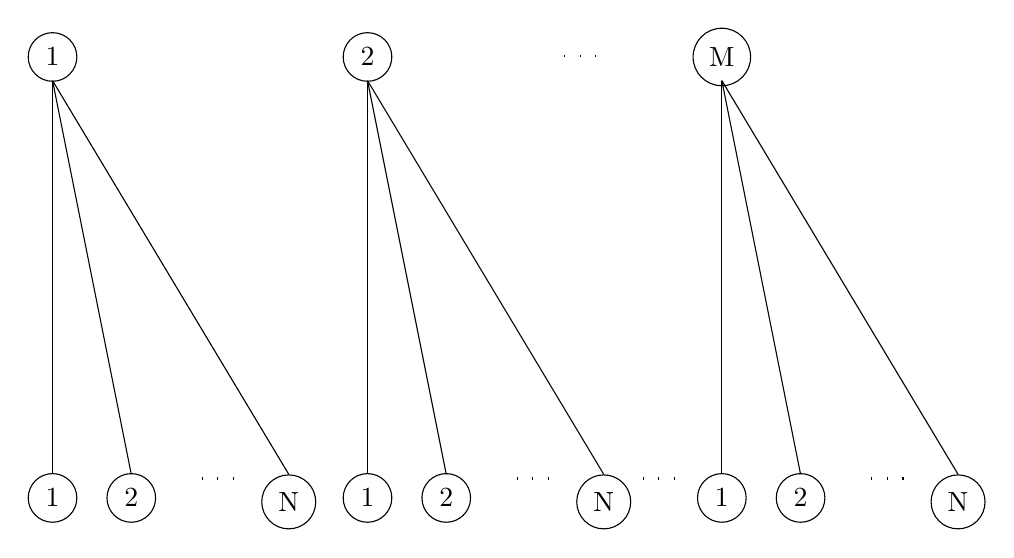
\begin{tikzpicture}
		\node[circle,draw] (c) at ((3.8, 5.3){1};
	%\draw (8.8, 5.1) circle (0.1cm) node[anchor=south] {0};
 	\draw (3.8, 5.0) -- (3.8, 0);
	\node[circle,draw] (c) at ((3.8, -0.3){1};
	%\draw (3.8, -0.1) circle (0.1cm)  node[anchor=north] {1};
 	\draw (3.8, 5.0) -- (4.8, 0);
	%\draw (5.8, -0.1) circle (0.1cm) node[anchor=north] {2};
	\node[circle,draw] (c) at ((4.8, -0.3){2};
 	\draw (3.8, 5.0) -- (6.8, 0);
	\node[circle,draw] (c) at ((6.8, -0.35){N};
	%\draw (13.8, -0.1) circle (0.1cm)  node[anchor=north] {N};
   	\draw (5.7, -2pt) -- (5.7, -1pt) ;
   	\draw (5.9, -2pt) -- (5.9, -1pt) ;
   	\draw (6.1, -2pt) -- (6.1, -1pt); 
   	
   	\node[circle,draw] (c) at ((7.8, 5.3){2};
	%\draw (8.8, 5.1) circle (0.1cm) node[anchor=south] {0};
 	\draw (7.8, 5.0) -- (7.8, 0);
	\node[circle,draw] (c) at ((7.8, -0.3){1};
	%\draw (3.8, -0.1) circle (0.1cm)  node[anchor=north] {1};
 	\draw (7.8, 5.0) -- (8.8, 0);
	%\draw (5.8, -0.1) circle (0.1cm) node[anchor=north] {2};
	\node[circle,draw] (c) at ((8.8, -0.3){2};
 	\draw (7.8, 5.0) -- (10.8, 0);
	\node[circle,draw] (c) at ((10.8, -0.35){N};
	%\draw (13.8, -0.1) circle (0.1cm)  node[anchor=north] {N};
   	\draw (9.7, -2pt) -- (9.7, -1pt) ;
   	\draw (9.9, -2pt) -- (9.9, -1pt) ;
   	\draw (10.1, -2pt) -- (10.1, -1pt); 
   	
   	\draw (11.3, -2pt) -- (11.3, -1pt) ;
   	\draw (11.5, -2pt) -- (11.5, -1pt) ;
   	\draw (11.7, -2pt) -- (11.7, -1pt); 
   	
   	\draw (10.3, 5.33) -- (10.3, 5.3) ;
   	\draw (10.5, 5.33) -- (10.5, 5.3) ;
   	\draw (10.7, 5.33) -- (10.7, 5.3); 
   	
   	\node[circle,draw] (c) at ((12.3, 5.3){M};
	%\draw (8.8, 5.1) circle (0.1cm) node[anchor=south] {0};
 	\draw (12.3, 5.0) -- (12.3, 0);
	\node[circle,draw] (c) at ((12.3, -0.3){1};
	%\draw (3.8, -0.1) circle (0.1cm)  node[anchor=north] {1};
 	\draw (12.3, 5.0) -- (13.3, 0);
	%\draw (5.8, -0.1) circle (0.1cm) node[anchor=north] {2};
	\node[circle,draw] (c) at ((13.3, -0.3){2};
 	\draw (12.3, 5.0) -- (15.3, 0);
	\node[circle,draw] (c) at ((15.3, -0.35){N};
	%\draw (13.8, -0.1) circle (0.1cm)  node[anchor=north] {N};
   	\draw (14.2, -2pt) -- (14.2, -1pt) ;
   	\draw (14.4, -2pt) -- (14.4, -1pt) ;
   	\draw (14.6, -2pt) -- (14.6, -1pt); 
\end{tikzpicture}
\caption{Consumer network}
\label{network}
\end{figure}

\subsection{Equilibria and intuition behind results} \label{results}

In setting up the structural model I aim to investigate first and foremost two separate effects, which reflect the WOM influence on the market. Not unlike learning-by-doing effects in \citet{Tirole}, I assume that investments in quality become less costly with the number of attracted consumers. This reflects one of the main features of software development markets, as the product is often discussed openly among developers, who are likely to report 'bugs' directly to the producer. The parameter $\alpha$ corresponds to such an effect. 
 
Secondly, I aim interested in the effect of delayed diffusion of information about goods on the market outcomes. In the baseline model I first look at the effect of the variable $N$, which corresponds to the number of consumers that were informed after the first period. In the extensions I add a number of dimensions to the consumer network, aiming to investigate the more complex effects of WOM. 

There are two possible states that incumbent finds herself in throught the game, which I will denote with $\gamma$. I define the state where the market is penetrated as a period of the game $G$, where the $m>0$, i.e. the information about the good reached consumers, who were not initially (and exoegenously) informed about the good and denote it as $\gamma=1$. In contrast, $\gamma=0$ is the period of the game when the incumbent is unknown to anybody, but the $M$ consumers informed about her existence in the beginning of the game. The game, thus, descibes the attempt of the incumbent to penetrate the market. As soon as $m>0$, she is successful. 

Starting from \textbf{second period} I define the maximisation problems of the incumbent and entrant. 
Because of the stric assumptions on cost, \textbf{in state 0} incumbent can not produce new quality, as she no longer has expected profit to draw from. She offers only products with $\{p_{12}, s_1\}$. Having not penetrated the market, she can only offer her goods to the same consumers as the entrant: the initial $M$. As this is the second and last period of the game, she does not expect additional profit from market penetration at this stage.

As the first-period good quality is set and the entrant can not produce quality herself, choosing between the incumbent's first-period good and the entrant's good the consumer will orient herself only to the price difference, resulting in Bertrand-type competition. Thus, both producers will set the price for the good of the quality $s_1$ equal to 0. As the incumbent does not offer a new version of the good her profit in this case is 0.

In contrast, in \textbf{state 1}, the incumbent has penetrated the market and can offer two versions of the good. As her first-period good and the entrant's good share the same quality, the competition is again Bertrand, resulting in both prices being set to zero.

Knowing this, the incumbent will optimally choose the quality development for the second-period good and the corresponding price using this profit equation:
$$\pi_2 =  (M+mN)p_2(1-\tfrac{p_2}{\Delta s}) - (w-\alpha m)\Delta s^2$$

The incumbent derives additional profit, compared to the first period, from $mN$ newly informed consumers. She offers them and the $M$ initially informed consumers both her first-period good and her newly developed product. Again, the competition between the incumbent's first-period good and the entrant's good results in the entrant striving to set the price below $p_e$ to compete with the incumbent's second period good. Incumbent's maximisation problem is:

$$\max_{p_2, s_2}   Mp_2(1-\tfrac{p_2 - p_e}{\Delta s}) + mN(1-\tfrac{p_2 - p_1}{\Delta s}) - (w-\alpha m)\Delta s^2$$

I demonstrate the interior solution in the appendix due to its length, and focus again on the special case, where the $p_1 = 0$. Instead of competing with both her own good and the entrant's good, the incumbent behaves as a monopolist. Her profit is: $(M(N+1))(1-\tfrac{p_1}{\Delta s})-(w-\alpha M)\Delta s^2$. Symmetrically to the above result, her optimal price is then: $p_2 = \tfrac{M(N+1)}{16(w-\alpha M)}$ and her development of quality $\Delta s = \tfrac{M(N+1)}{8(w-\alpha M)}$.

Using the results above I set up the maximisation problem in \textbf{the first period}. The problem itself will not be used in the empirical model, however, it allows me to derive the conditions, under which the incumbent does set the price 0 in the first period and use this equation to calculate the probability of it being 0 in the first period, which I will use to select the sample of observations for the regression. 

(first period profit equation missing)

\subsection{Discussion}\label{intuition}

The majority of model implications seem intuitive. The bigger the market, the higher the speed of information diffusion and the higher the feedback effect, the more incentive the producer has to develop quality, once she penetrates the market. Keeping the price of the first-period good fixed and equal to 0, the incumbent, who is aware of the feedback effect, ensures both that the competing good will not be tried out by the initially informed consumers, while reaping the benefits of having penetrated the market with complete certainty. 

My goal is to explore the welfare implications of this quality development decision. (need the solution for the first period model)

\subsection{Testable Implications and Comparative Statics}

By model prediction, when the price is equal to 0, all consumers who are initially informed about the incumbent's good, buy it. Being able to see the overall number of downloads, which is equal to $\tfrac{1}{2}(MN+M) + M$ I can derive $M$, which I will use as an estimate of demand.  

\textbf{Available Data:} 

The dataset is drawn from two separate software development forums in US and Russia. Each dataset contains cross-sectional observations on a product developed within the forum. I collect the initial price at launch ($p_1$) of the product and the current price ($p_2$) in local currency and divide it by the corresponding price index at the country of launch. The developer's rank at the date of launch ($w$) and currently ($w-\alpha$) are available at the product page. To estimate $N$ I collect the number of product mentions outside of the product page using the search engine of the website. Lastly, I calculate the response rate on opened issues in GitHub to calculate the quality development of the product since launch ($\Delta s$).

As this approach implies that different products have longer timelines, I apply different discounting methods to all variables, except price, and compare the estimation results. 

(Here will be a chunk of text describing data and its extraction).



\textbf{Part 1:} Identify succesful market penetration.

Using the condition on the first-period price, I run a regression of probability of each specific firm setting a price 0, and select a sample of firms, for whom this fitted probability is low.

\textbf{Part 2:} Estimate the effect of the parameters of interest.

Once I have a set of firms, who have successfully entered the market, I use nonlinear OLS to estimate the equation for development of software quality. The sensitivity of results can be checked by using the data from two different software developer forums, as well as by introducing a number of fixed parameters. 

\textbf{Part 3:} using the restrictions on the exogeneous parameters from the first period model I can compare how the model performs in the simulations with different $\beta$ values to the parameters (mainly, $N$) that I observe. I compare these results with the simulations for a model with no feedback effects and show which ones are closer to the real value of N.

\textbf{Comparative Statics}
\begin{itemize}
    \item various WOM network properties:
    compare the WOMs of the two forums and simulate different structures;
    \item demand shock: 
    model the counterfactual and check how the results compare from the effects from the Google Play Store paid app restrictions towards Russian users;
    \item supply shock: 
    model the counterfactuals and check how the results coincide with the effects from influx of members to PDA Forums after sanctions on Google Play Store on the side of developers;
    \item shock of feedback effect (blockage of GitHub for Russian software developers): compare the predictions of the model against the real impact.
\end{itemize}
%\section{Conclusion}

\subsection{Extensions}

%\subsubsection{Incumbent Offers a Menu:}

%instead of disallowing access of new consumers to her first period good, incumbent offers it as an alternative to the second period version for consumer 0. In \textbf{state 1} her maximisation problem is:

%$$\pi_2 = Np_2(1-\tfrac{p_2-p_1}{\Delta s}) - (w-\alpha)\Delta s^2 + p_1(\tfrac{p_2s_1-p_1s_2}{s_1\Delta s})$$

%After taking the derivative, it becomes possible to formulate the solution in terms of $p_2$ and $\Delta s$, instead of two separate qualities. Unfortunately, due to market sizes being different, the FOC for equilibrium quality is described with a third degree polynomial:

%$$\tfrac{N}{4} + \tfrac{(1+N)p_1}{2\Delta s} - \tfrac{p_1^{2inc}(1-N)^2}{4N\Delta s^2} - 2 \Delta s (w-\alpha)=0$$

%While there is only one real solution to this equation, it is not very informative. Interestingly, however, it collapses to that of the baseline model, if $p_1 = 0$. 


I now investigate the repercussions of different network formation assumptions on the model results.
 \subsubsection{Different Information Diffusion Assumption:}

    Assume the probability of recommending a good after buying is not 1, but a function of the goods quality or price.
    
    It may happen that people in general are more likely to talk about the good if it's cheap, or if the quality is high, or if they perceive the price to be low for this level of quality (i.e. reacting to quality-to-price ratio). Moreover, if experts in general are more likely to recommend the good, then targeting consumers with high valuation of quality by producing high quality good with lower prices may compensate the incumbent's investment in the quality. development.
    
    Empirics:  Fit a linear function instead of relying on demand.
    
    \subsubsection{Homophily or heterophily of networks:}
    
    In real-world networks homophily is generally more widespread, meaning people are more likely to be friends with similar people. In the model I assumed that the N consumers brought by the consumer 0 have a uniform valuation of the quality of good. However, it may be true that being somebody who appreciates quality of the software highly, consumer 0 is more likely to bring more consumers like herself, whose valuation for quality is also high.
    
    In contrast, heterophily of the network may occur, for example, if consumers who value quality are more likely to post reviews on the forum, which will be read by novices, who are less likely to be interested in more in-depth discussions of specific software and do not value the quality so much.
    
    Assume that consumers are divided into two types in their communication. High-type consumers value quality more than average: $\theta_h\geq 0.5$, whereas low type consumers do not value it so much. $\theta_l < 0.5$.  It is evident that if the producer is aware of the underlying properties of the network, e.g. homophily or heterophily, she can use that information to price discriminate second period consumers.  
 \subsubsection{Clustering of consumers and small-world networks:}
M consumers in the first period forming clusters.




\newpage
\bibliography{bibliography}

\end{document}
